%-*- coding:utf-8 -*-

\documentclass[10pt,dvipdfmx]{beamer}
\usepackage{tutorial}

\title{計算機実験II (L4) --- 多体系の量子力学}
\date{2020/10/23}

\begin{document}

\begin{frame}
  \titlepage
  \tableofcontents
\end{frame}

\begin{frame}[t]{講義日程}
  \begin{itemize}
    % \setlength{\itemsep}{1em}
  \item 全8回 (金曜5限 {\color{red}17:05}-18:35)
    \begin{itemize}
    \item {\color{gray} 10月8日 第1回: 乱択アルゴリズム、モンテカルロ法}
    \item 10月15日 第2回: 多体系の統計力学、マルコフ連鎖モンテカルロ法
    \item 10月22日 第3回
    \item 10月29日 第4回
    \item 11月5日 休講 (もくもく会)
    \item 11月12日 休講 (物理学教室コロキウム)
    \item 11月19日 第5回
    \item 11月26日 休講 (物理学教室コロキウム)
    \item 12月3日 第6回
    \item 12月10日 第7回
    \item 12月17日 休講 (物理学教室コロキウム)
    \item 12月24日 第8回
    \item 1月7日 休講 (もくもく会)
    \item 1月18日(火) 休講 (予備日)
    \end{itemize}
  \end{itemize}
\end{frame}


\section{対角化 (復習)}
\begin{frame}[t,fragile]{シュレディンガー方程式の行列表示}
  \begin{itemize}
    %\setlength{\itemsep}{1em}
  \item シュレディンガー方程式
    \[
    [-\frac{d^2}{dx^2}+V(x)]\psi(x) = E \psi(x)
    \]
  \item 連立差分方程式を行列の形で表す($\psi(x_0)=\psi(x_n)=0$)
    \begin{footnotesize}
    \[
    \begin{pmatrix}
      \frac{2}{h^2}+V(x_1) & -\frac{1}{h^2} \\
      -\frac{1}{h^2} & \frac{2}{h^2}+V(x_2) & -\frac{1}{h^2} \\
      & -\frac{1}{h^2} & \frac{2}{h^2}+V(x_3) & -\frac{1}{h^2} \\
      & & \ddots & \ddots \\
      & & & -\frac{1}{h^2} & \frac{2}{h^2}+V(x_{n-1}) \\
    \end{pmatrix}
    \begin{pmatrix}
      \psi(x_1) \\
      \psi(x_2) \\
      \psi(x_3) \\
      \vdots \\
      \psi(x_{n-1}) \\
    \end{pmatrix}
    = \cdots % E
    %% \begin{pmatrix}
    %%   \psi(x_1) \\
    %%   \psi(x_2) \\
    %%   \psi(x_3) \\
    %%   \vdots \\
    %%   \psi(x_{n-1}) \\
    %% \end{pmatrix}
    \]
    \end{footnotesize}
  \item $(n-1) \times (n-1)$の疎行列の固有値問題
    \begin{itemize}
    \item 固有値: 固有エネルギー
    \item 固有ベクトル: 波動関数
    \end{itemize}
  \end{itemize}
\end{frame}

\begin{frame}[t,fragile]{固体物理・量子統計物理に現れる行列}
  \begin{itemize}
    %\setlength{\itemsep}{1em}
  \item 強束縛近似(tight-binding approx.)のもとでの第二量子化表示
    \[
    H = -t \sum_{\langle i,j \rangle \sigma} (c_{i,\sigma}^\dagger c_{j,\sigma} + h.c.) + \text{(相互作用)}
    \]
  \item 局所スピン模型(ハイゼンベルグ模型)
    \[
    H = -J\sum_{\langle i,j \rangle} S_i \cdot S_j
    = -J\sum_{\langle i,j \rangle} [S_i^z S_j^z +\frac{1}{2} (S_i^+ S_j^- + S_i^- S_j^+) ]
    \]
  \item 格子点の数を$n$とすると、ハミルトニアンはそれぞれ$4^n \times 4^n$、$2^n \times 2^n$の(疎)行列で表される。
  \item $n$が大きくなると、行列の次元は指数関数的に増加
  \item 量子多体系に共通する困難
  \end{itemize}
\end{frame}

\begin{frame}[t,fragile]{行列の数値対角化}
  \begin{itemize}
    %\setlength{\itemsep}{1em}
  \item 一般的に次元が5以上の行列の固有値は、あらかじめ定まる有限回の手続きでは求まらない
    \begin{itemize}
    \item 必ず何らかの反復法(+収束判定)が必要となる
    \end{itemize}
  \item 密行列向きの方法
    \begin{itemize}
    \item Jacobi法
    \item Givens変換・Householder法(三重対角化) + QR法など
    \end{itemize}
  \item 疎行列向きの方法
    \begin{itemize}
    \item べき乗法
    \item Lanczos法(三重対角化) + QR法など
    \end{itemize}
  \item 固有ベクトル
    \begin{itemize}
    \item QR法で求めたものを逆変換
    \item 逆反復法で精度改善
    \end{itemize}
  \end{itemize}
\end{frame}


% -*- coding: utf-8 -*-

\section{横磁場イジング模型}

\begin{frame}[t,fragile]{横磁場イジング模型}
  \begin{itemize}
    %\setlength{\itemsep}{1em}
  \item ハミルトニアン($2^N \times 2^N$行列)
    \[
      H = H_z + H_x = - J \sum_{\langle i,j \rangle} \sigma_i^z \sigma_j^z - h \sum_i \sigma_i^z - \Gamma \sum_i \sigma_i^x
    \]
  \item $\sigma_i^x$、$\sigma_i^z$: パウリ行列($2 \times 2$行列)
    \begin{align*}
      \big(\sigma_i^z\big)^2 &= \big(\sigma_i^x\big)^2 = I \\
      [ \sigma_i^z, \sigma_i^x ] &\ne 0
    \end{align*}
  \item $J$: スピン間の相互作用($J>0$: 強磁性、$J<0$: 反強磁性)
  \item $h$: 縦磁場(準位間のエネルギー差$=2h$)
  \item $\Gamma$: 横磁場(トンネリング)
  \item 以降、$\sigma_i^z$を対角化する基底($|\!\uparrow\rangle_i$, $|\!\downarrow\rangle_i$)で考える
  \end{itemize}
\end{frame}

\begin{frame}[t,fragile]{横磁場イジング模型}
  \begin{itemize}
    %\setlength{\itemsep}{1em}
  \item 2サイト系
    \[
      H = -J \sigma_1^z \sigma_2^z - h (\sigma_1^z + \sigma_2^z) - \Gamma (\sigma_1^x + \sigma_2^x)
    \]
  \item 行列要素
    \begin{align*}
      \langle \uparrow \uparrow \!| H |\! \uparrow \uparrow \rangle &= -J - 2h \\
      \langle \uparrow \uparrow \!| H |\! \uparrow \downarrow \rangle &= -\Gamma \\
      \langle \uparrow \uparrow \!| H |\! \downarrow \downarrow \rangle &= 0 \\
      &\vdots
    \end{align*}
  \end{itemize}
\end{frame}

\begin{frame}[t,fragile]{量子相転移}
  \begin{itemize}
    %\setlength{\itemsep}{1em}
  \item $h=0$の場合
    \begin{itemize}
    \item $\Gamma \rightarrow 0$: $|\!\uparrow\uparrow\cdots\uparrow\rangle$、あるいは$|\!\downarrow\downarrow\cdots\downarrow\rangle$が基底状態(二重縮退)
    \item $J \rightarrow 0$: $\sigma_i^x$の固有状態($|\!\uparrow\rangle_i + |\!\downarrow\rangle_i$)の積が基底状態(全ての状態の重ね合わせ)
    \end{itemize}
  \item 一次元系
    \[
      H = - J \sum_{i} \sigma_i^z \sigma_{i+1}^z - \Gamma \sum_i \sigma_i^x
    \]
    $\Gamma = J$で量子相転移(熱ゆらぎではなく量子ゆらぎによる相転移)  
  \end{itemize}
\end{frame}


\section{多体量子系の時間発展}

\begin{frame}[t,fragile]{横磁場イジング模型の時間発展}
  \begin{itemize}
    %\setlength{\itemsep}{1em}
  \item 時間依存シュレディンガー方程式の形式解
    \[
    \Psi(t) = e^{-iHt} \Psi(0)
    \]
    \begin{itemize}
    \item 有限差分法、クランク・ニコルソン法
    \end{itemize}
  \item 鈴木・トロッター分解 ($\Delta t = t / M$)
    \begin{align*}
      e^{-iHt} &= \big[ e^{-iH\Delta t} \big]^M \approx \big[ e^{-iH_z\Delta t} e^{-iH_x\Delta t} \big]^M \\
      &= \big[ e^{i\Delta t J \sum_{\langle i,j \rangle} \sigma_i^z \sigma_j^z} e^{i\Gamma \sigma_1^x\Delta t} e^{i\Gamma \sigma_2^x\Delta t} \cdots e^{i\Gamma \sigma_N^x\Delta t} \big]^M
    \end{align*}
    (さらに$e^{-iH\Delta t} \approx e^{-iH_z\Delta t/2} e^{-iH_x\Delta t} e^{-iH_z\Delta t/2}$と対称に分解すると近似の次数が上がる)
  \item $[\sigma_i^x]^2 = I$より
    \[
    e^{i\Gamma \sigma_i^x\Delta t} = \cos (\Gamma\Delta t) + i \sigma_i^x \sin (\Gamma\Delta t)
    \]
  \end{itemize}
\end{frame}

\begin{frame}[t,fragile]{量子アニーリング}
  \begin{itemize}
    %\setlength{\itemsep}{1em}
  \item 離散最適化問題
    \[
    H = -J \sum_{i<j} \epsilon_{ij} \sigma_i^z \sigma_j^z
    \]
    の基底状態配位と基底状態エネルギーを求めたい
    \begin{center}
      \resizebox{0.6\textwidth}{!}{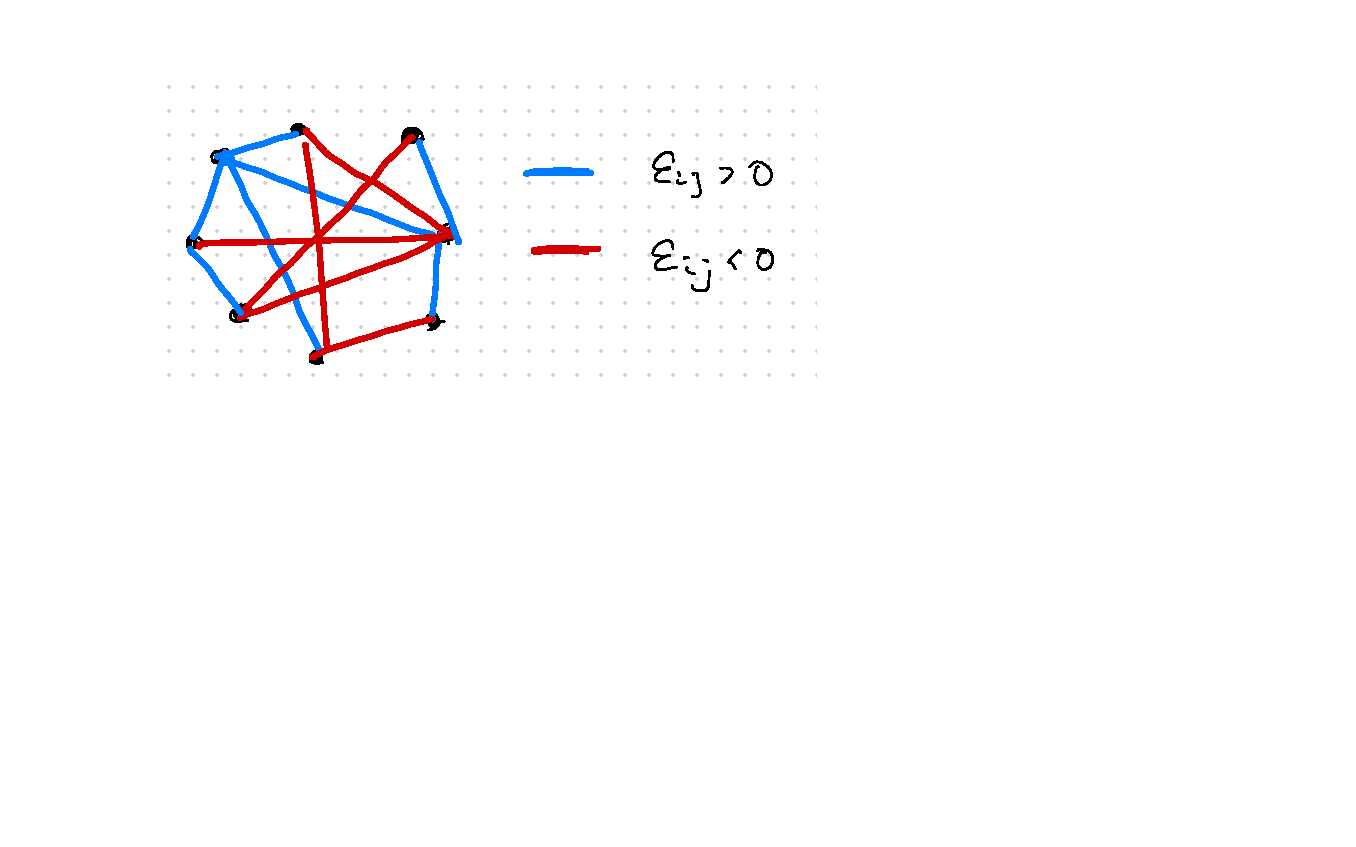
\includegraphics{image/spinglass.pdf}}
    \end{center}
  \end{itemize}
\end{frame}

\begin{frame}[t,fragile]{量子アニーリング}
  \begin{itemize}
    %\setlength{\itemsep}{1em}
  \item 横磁場を導入
    \[
    H = -J \sum_{i<j} \epsilon_{ij} \sigma_i^z \sigma_j^z - \Gamma \sum_i \sigma_i^x
    \]
  \item 古典極限 ($J=1$, $\Gamma=0$)
    \begin{itemize}
    \item 求めたい基底状態
    \end{itemize}
  \item 量子極限 ($J=0$, $\Gamma=1$)
    \begin{itemize}
    \item $2^N$個の全ての状態の重ね合わせ
    \end{itemize}
  \item 量子アニーリング
    \begin{itemize}
    \item $J+\Gamma=1$を保ったままで、$\Gamma=1$から$\Gamma=0$まで「ゆっくり」と減少させながら時間発展させる
      \[
      J = 1-\Gamma = t/T \qquad (0 \le t \le T)
      \]
    \item $T \rightarrow \infty$の極限で確率1で基底状態に収束
    \end{itemize}
  \end{itemize}
\end{frame}


\section{量子コンピュータ}

\begin{frame}[t,fragile]{量子コンピュータと量子ゲート}
  \begin{itemize}
    %\setlength{\itemsep}{1em}
  \item (ゲート型)量子コンピュータ

    $N$量子ビットに対して、量子ゲートにより状態を操作

    \begin{itemize}
    \item 「量子ビット」= 2準位系($S=1/2$スピン) \ $|0\rangle=|\!\uparrow\rangle, |1\rangle=|\!\downarrow\rangle$
    \item 「量子ゲート」= 少数量子ビットに対するユニタリ変換
    \end{itemize}
  \item 1量子ビットゲート
    \begin{itemize}
    \item Xゲート(量子NOT)
      \[
      X = \begin{pmatrix} 0 & 1 \\ 1 & 0 \end{pmatrix} = \sigma^x
      \]
    \item Rzゲート($z$軸まわりの回転)
      \[
      Rz(\theta) = \begin{pmatrix} e^{-i\theta/2} & 0 \\ 0 & e^{i\theta/2} \end{pmatrix} = e^{-i\theta\sigma^z/2}
      \]
    \item アダマールゲート
      \[
      H = \frac{1}{\sqrt{2}} \begin{pmatrix} 1 & 1 \\ 1 & -1 \end{pmatrix} = \frac{1}{\sqrt{2}} (\sigma^x + \sigma^z)
      \]
    \end{itemize}
  \end{itemize}
\end{frame}

\begin{frame}[t,fragile]{量子ビットゲート}
  \begin{itemize}
    %\setlength{\itemsep}{1em}
  \item 2量子ビットゲート
    \begin{itemize}
    \item CXゲート(制御NOT)
      \[
      CX = \begin{pmatrix} 1 & 0 & 0 & 0 \\ 0 & 1 & 0 & 0 \\ 0 & 0 & 0 & 1 \\ 0 & 0 & 1 & 0 \end{pmatrix}
      \]
    \end{itemize}
  \item 3量子ビットゲート
    \begin{itemize}
    \item CCXゲート(トフォリゲート)
      \[
      CCX = \begin{pmatrix}
        1 & 0 & 0 & 0 & 0 & 0 & 0 & 0 \\
        0 & 1 & 0 & 0 & 0 & 0 & 0 & 0 \\
        0 & 0 & 1 & 0 & 0 & 0 & 0 & 0 \\
        0 & 0 & 0 & 1 & 0 & 0 & 0 & 0 \\
        0 & 0 & 0 & 0 & 1 & 0 & 0 & 0 \\
        0 & 0 & 0 & 0 & 0 & 1 & 0 & 0 \\
        0 & 0 & 0 & 0 & 0 & 0 & 0 & 1 \\
        0 & 0 & 0 & 0 & 0 & 0 & 1 & 0 \end{pmatrix}
      \]
    \end{itemize}
  \end{itemize}
\end{frame}

\begin{frame}[t,fragile]{量子加算器}
  \begin{itemize}
    %\setlength{\itemsep}{1em}
  \item 1量子ビットの加算 $\Rightarrow$ CCXゲートとCXゲートで実現できる
    \begin{center}
      \resizebox{0.5\textwidth}{!}{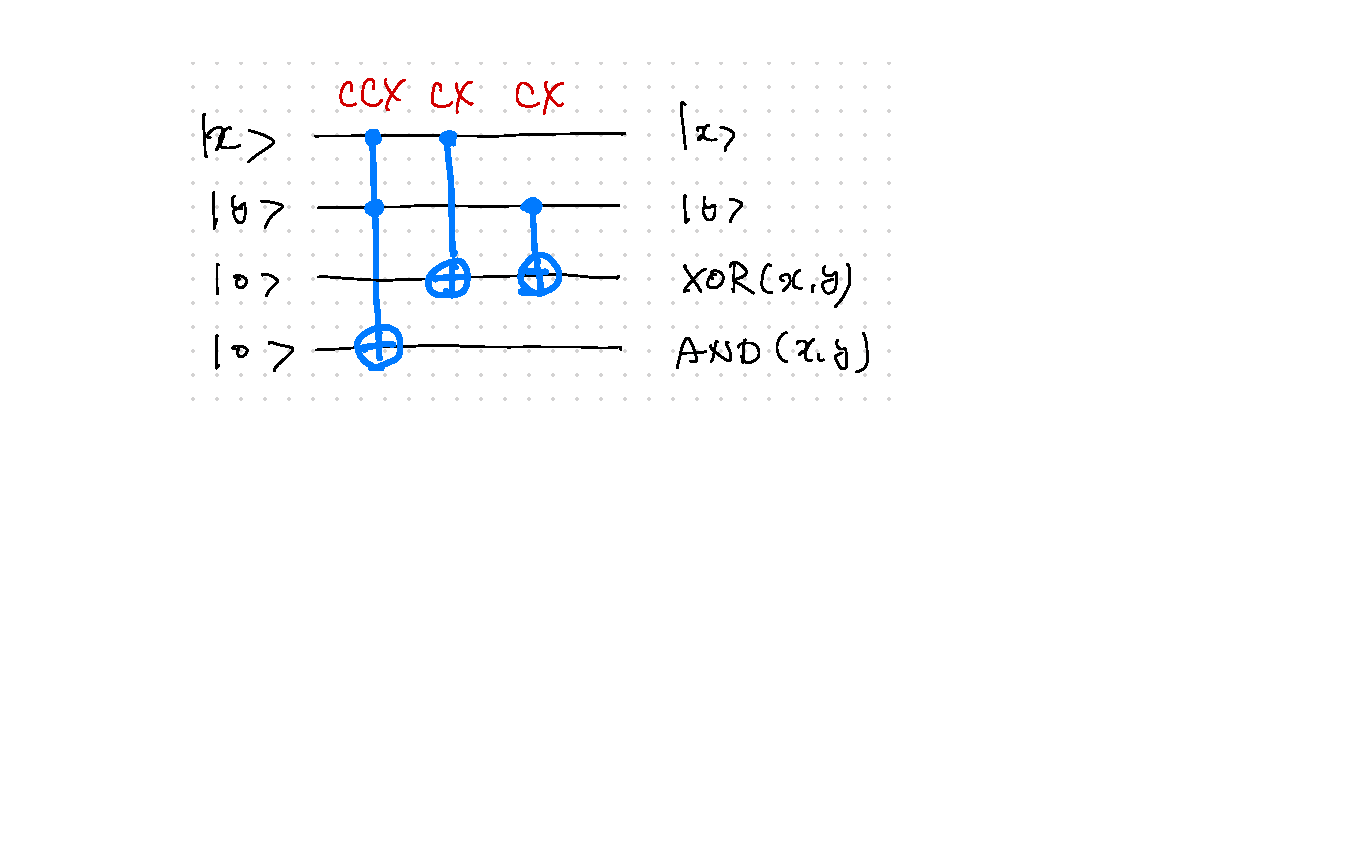
\includegraphics{image/adder1.pdf}}
    \end{center}
  \item CCXゲートは、Hゲート、Rzゲート、CXゲートの組み合わせで表現できる
  \item 任意の量子回路は、Hゲート、Rzゲート、CXゲートの組み合わせで表現できる (万能量子ゲート)
  \end{itemize}
\end{frame}

\begin{frame}[t,fragile]{量子加算器}
  \begin{itemize}
    %\setlength{\itemsep}{1em}
  \item 3量子ビット加算器
    \begin{center}
      \resizebox{0.6\textwidth}{!}{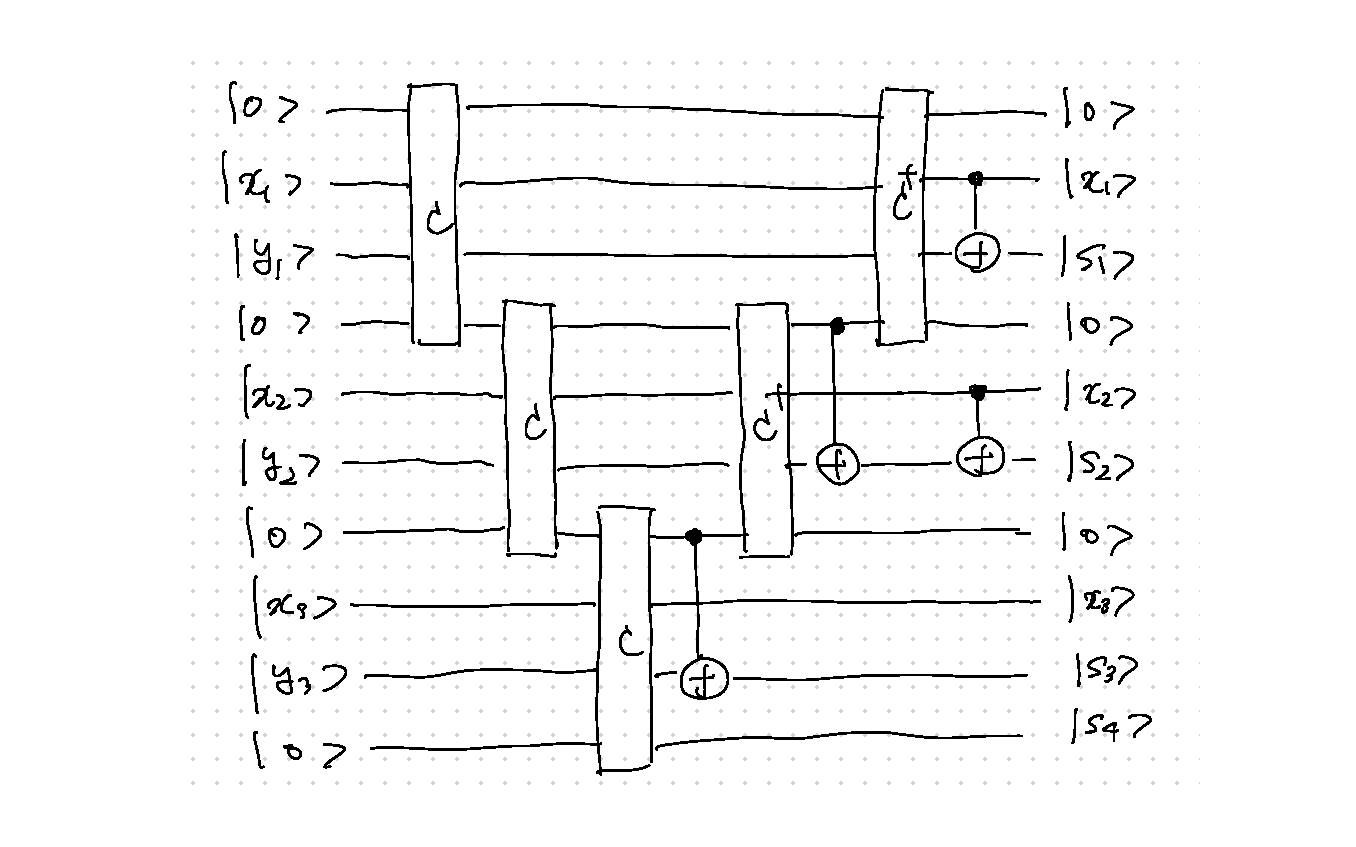
\includegraphics{image/adder3.pdf}}
      \resizebox{0.35\textwidth}{!}{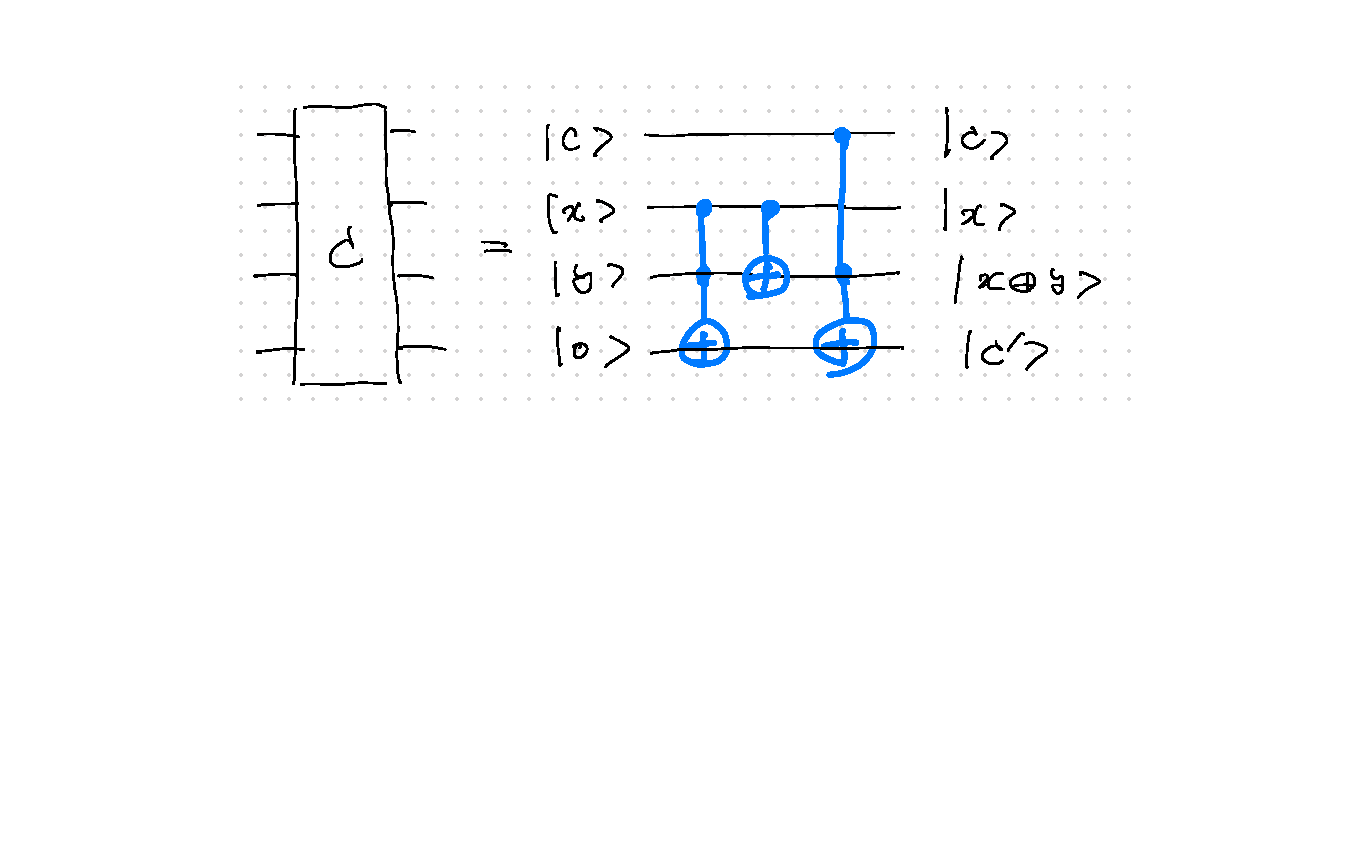
\includegraphics{image/adder2.pdf}}
    \end{center}
  \end{itemize}
\end{frame}



\section{}
\begin{frame}[t]{本日の課題}
  \begin{itemize}
    %\setlength{\itemsep}{1em}
  \item 実習
    \begin{itemize}
    \item C言語におけるベクトル・行列の扱いの復習 (計算機実験I 第4回)
    \item 密行列の対角化の復習 (計算機実験I 第6回)
    \item (疎行列の対角化の復習 (計算機実験I 第7回))
    \item 実習課題一覧\href{https://github.com/todo-group/ComputerExperiments/releases/tag/2020a-computer2}{exercise-2.pdf}から対角化(あるいは別の)課題を選び実習
    \end{itemize}
  \item 質問はSlackの「\# 5\_対角化」あるいは他の適当と思われるチャンネルで
  \item 今回は「作業レポート」はなし
  \item 「レポートNo.1」 (ITC-LMSを参照) 締切 2020/11/6(金)
  \end{itemize}
\end{frame}

\end{document}
